%% CAPITULO 1
\hypertarget{estilo:capitulo}{}
\chapter{INTRODUÇÃO} 

A precipitação é uma variável que influencia os estados presente e futuro da atmosfera,  principalmente na região tropical e sua previsão sobre esta região  se constitui como um grande desafio para a Previsão Numérica de Tempo (PNT). Os processos diabáticos são dominantes nesta região e desempenham um papel importante na determinação dos padrões convectivos, na formação de chuvas e tempestades através da geração e distribuição de calor e energia nos movimentos verticais e horizontais. Estes processos são de escala subgrade e sua representação pelos modelos de PNT é feita através de parametrizações  físicas. Há vários tipos de parametrizações que são mais adequadas em relação às escalas espacial e temporal desses fenômenos.

Na modelagem atmosférica, o aprimoramento do desempenho da PNT de curto e médio prazo depende não somente do poder computacional envolvido - computadores cada vez mais rápidos e eficientes, mas também do conhecimento das leis que governam o movimento da atmosfera. Embora não se tenha um conhecimento total sobre estas leis, pois a atmosfera possui um comportamento caótico, os modelos de previsão de tempo são construídos com base em leis gerais que descrevem o escoamento atmosférico. Desta forma, os modelos de PNT mantêm uma forte dependência em relação ao estado inicial, o qual é importante para a qualidade da previsão. Este estado inicial - a Análise, é determinante para a PNT: quanto mais realística, quanto mais informações possuir sobre a atmosfera em seu instante de análise, melhor será o resultado da previsão. Uma forma de aprimorar o desempenho dos modelos de PNT é incluir dados de precipitação no processo de assimilação.

\citeonline{krishnamurtietal91} e \citeonline{nunesroads05} apontam para o fato de que uma previsão acurada de precipitação na região dos trópicos está diretamente relacionada com a qualidade dos campos iniciais de temperatura e umidade do solo – parâmetros que influenciam diretamente os estados da atmosfera, sem os quais os fluxos de calor necessários para a correta simulação/composição da estrutura vertical das nuvens convectivas é comprometida. Nesse sentido, a assimilação de precipitação tem sido proposta como uma forma de melhorar a representação destes campos iniciais permitindo que a representação da convecção, a formação de nuvens e a precipitação sejam mais realísticas. Como consequência do aprimoramento desses campos iniciais, tem-se a redução do tempo de \textit{spin up} (uma vez que os campos iniciais de massa e vento utilizados para a geração da análise já estão balanceados), o incremento da qualidade das análises globais e das previsões de curto prazo sobre os trópicos \cite{heckleyetal90}; \cite{falkovichetal00}. Vários trabalhos mostram também que a utilização da assimilação de precipitação para a inicialização dos modelos é mais substancial para previsões de curto prazo, uma vez que esta é vinculada às parametrizações físicas (como esquemas de convecção) e aos erros sistemáticos dos modelos \cite{kasaharaetal94}; \cite{mathur95}; \cite{zupanskimesinger95}; \cite{nunescocke04}.

A Assimilação de Dados (AD) constitui um conjunto de técnicas e ferramentas estatísticas cujo principal objetivo é a determinação da análise para uso como condição inicial dos modelos de PNT. Segundo \citeonline{talagrand97}, a AD pode ser definida como uma técnica acurada para reconstruir o escoamento atmosférico utilizando todas as informações disponíveis no momento de sua geração. Estas informações englobam observações convencionais (superfície e ar superior) e não convencionais (como dados obtidos a partir de satélites) que combinados de forma ótima com os campos iniciais (\textit{first guess}) produzidos por um modelo de PNT, são capazes de gerar uma estimativa muito próxima do escoamento atmosférico observado \cite{kalnay03}.

Historicamente, a AD vem evoluindo de simples técnicas empíricas de interpolação de dados no início da década de 1950 (Análise Simples, Correções Sucessivas \cite{cressman59}, Relaxação Newtoniana - \textit{Nudging}), a sofisticados procedimentos estatísticos-dinâmicos (Interpolação Ótima - uso combinado de observações e modelagem), desenvolvidos na última década do século passado. Estas técnicas foram desenvolvidas com base na teoria da estimação, a partir da qual originaram-se técnicas mais modernas baseadas no Filtro de Kalman (EnKF - \textit{Ensemble Kalman Filter}; LEKF - \textit{Local Ensemble Kalman Filter}; LETKF – \textit{Local Ensemble Transform Kalman Filter}) e métodos variacionais em 3 ou 4 dimensões (3DVar e 4DVar). Todos esses esquemas de análise estão consolidados sobre uma base estatística, e a diferença básica entre eles está no modo com que cada abordagem produz a análise, combinando de formas diferentes o \textit{first guess} e as observações \cite{kalnay03}.

A assimilação de dados de alta resolução espacial e temporal também contribui para estudos diagnósticos detalhados e a produção de reanálises atmosféricas de alta qualidade. Vários trabalhos \cite{cavalcantiherdies04}; \cite{herdiesetal06}; \cite{rozantecavalcanti07}; \cite{herdiesetal07}; \cite{skabarnicolini09} mostram que a assimilação de dados do projeto \textit{South America Low-Level Jet Experiment} (SALLJEX) tem grande impacto nas análises produzidas por modelos globais e regionais e nas previsões de curto prazo produzidas a partir destas análises. As análises geradas por estes experimentos contêm um nível maior de detalhamento das variáveis meteorológicas e contribuem para a descrição mais real de fenômenos de mesoescala como Jatos de Baixos Níveis (JBN) e Sistemas Convectivos de Mesoescala (SCMs). 

A importância destes estudos de campo demonstra que a inclusão de um número maior de dados observacionais no processo de assimilação de dados, é imprescindível para a melhorar qualidade das análises regionais e globais que são utilizadas operacionalmente em diversos centros de PNT e em outros estudos. De outra forma, projetos que tem por objetivo a criação de reanálises também contribuem para a qualidade de trabalhos de pesquisa, seja em estudos de validação de modelos ou estudos diagnósticos que buscam detalhar processos físicos relacionados principalmente à convecção e à precipitação sobre os trópicos. 

Entre esses projetos, pode-se destacar as reanálises regionais tais como o \textit{North American Regional Reanalysis} (NARR) do NCEP \cite{messingeretal06} cujo objetivo foi prover uma reanálise em alta resolução sobre a região continental dos Estados Unidos, a Reanálise de 40 Km do CPTEC \cite{aravequiaetal07} com a qual foi criada uma reanálise regional de cinco anos (de 2000 a 2004) sobre a região continental da América do Sul (AS) utilizando todos os dados disponíveis de superfície e ar superior. Entre outros pode-se também citar as reanálises globais do NCEP (versões 1 - \citeonline{kalnayetal96} e 2 - \citeonline{kanamitsuetal02}), a do \textit{European Centre for Medium Range Weather Forecasts} (ECMWF), denominada Era-40 (que é uma reanálise de 45 anos - \citeonline{upalaetal05}). Além disso, trabalhos que utilizaram a assimilação de dados gerando análises simples, seja utilizando a Inicialização Física (IF) \cite{nunescocke04}; \cite{biazettoetal05} ou \textit{nudging}, têm sua importância destacada porque demonstram a capacidade de gerar análises de qualidade utilizando metodologias mais simples e que se mostram promissoras. 

No caso do \textit{nudging} (ou Relaxação Netoniana), no período que antecede a previsão as variáveis do modelo são conduzidas em direção às observações através de termos adicionais nas equações prognósticas. Quando se chega ao tempo de previsão, estes termos adicionais são removidos e a previsão é feita utilizando-se as componentes originais do modelo. Esta técnica coloca o modelo e as observações em harmonia e, em relação à IF, tem a vantagem de produzir um estado inicial relativamente balanceado e livre de ruído meteorológico. Com isso, os ganhos podem ser maiores visto que o estado inicial produzido pelo modelo está mais próximo do observado. Na IF, verifica-se que os maiores ganhos estão nas primeiras horas de previsão, uma vez que não se utilizam termos forçantes para controlar as variáveis do modelo. Neste caso, as modificações feitas estão na parametrização convectiva (caso em que inverte-se a parametrização \textit{Cumulus} a fim de se obter um modelo linearizado transposto) cuja vantagem está no controle dinâmico das variáveis.

A análise objetiva e a inicialização são os componentes principais dos sistemas de AD. Segundo \citeonline{kasahara90}, os métodos de análise são projetados para calcular os campos de massa e a componente rotacional do vento. Já os de inicialização são desenhados para obter a componente irrotacional do vento e o campo de velocidade vertical associado, os quais são balanceados com os campos de massa e devem ser livres de ruído meteorológico (ondas espúrias). A teoria quase-geostrófica, Método dos Modos Normais Não-Lineares e outros produzem bons resultados em latitudes médias \cite{krishnamurtietal91}, mesmo sem considerar os efeitos diabáticos para movimentos de grande escala. Nos trópicos, entretanto, devido à pequena magnitude do parâmetro de Coriolis e ao fraco gradiente horizontal de temperatura, a situação é diferente: os métodos de inicialização devem incluir os efeitos diabáticos, associados principalmente à precipitação. A técnica de \textit{nudging} oferece uma interface interessante para a inclusão destes efeitos sem requerer nenhum outro processo de inicialização para se manter o balanço dinâmico.

Os benefícios da assimilação de dados de precipitação têm sido demonstrados há alguns anos em experimentos com inicialização diabática e \textit{nudging} \cite{zupanskimesinger95}. De forma similar, a IF é também uma técnica de inicialização, mas com a necessidade de utilizar um modelo adjunto para assimilação e um filtro para o controle das ondas espúrias. No \textit{nudging}, isto não é necessário, visto que a única direção em que os termos artificiais das equações prognósticas podem seguir é o das observações.

Por outro lado a combinação de assimilação variacional e inicialização \cite{zupanskimesinger95}; \cite{treadon96} apresenta uma solução matematicamente elegante e oferece uma estrutura natural para a assimilação da precipitação. Embora esta combinação mostre-se atraente do ponto de vista científico, possui um custo de desenvolvimento e manutenção muito elevados. Isso implica na utilização de um modelo adjunto utilizado para assimilação ou, no caso da assimilação de precipitação, a inversão da parametrização convectiva. Estes modelos adjuntos aumentam o tempo de processamento da análise e nem sempre são de simples determinação. Seu cálculo inclui a solução de um problema inverso, o que é complicado do ponto de vista matemático, pois é altamente não linear - a  PNT sendo tratada como um problema inverso inclui uma série de aproximações que não satisfazem por completo a solução do problema em si. A solução deste problema também é dificultada pelo custo envolvido, pois exige o conhecimento dos algoritmos envolvidos nos esquemas de assimilação e dinâmica/física dos modelos, além de computadores potentes o suficiente para suprir o custo computacional.

No CPTEC, o atual sistema operacional de AD é o \textit{Physical-space Statistical Analysis System} (PSAS) T213L42 – com 213 ondas no Equador e 42 níveis verticais sigma (~60 km de resolução horizontal). Para a geração das análises regionais, é utilizado o \textit{Regional} PSAS (RPSAS) que é a versão regional do sistema PSAS desenvolvido pela divisão de assimilação de dados da \textit{National Aeronautics and Space Administration} (NASA) \cite{dasilvaetal95}; \cite{courtier97}. Este sistema é usado operacionalmente para produzir a análise utilizada pelos modelos regionais do centro (Eta nas versões 40 e 20 km). Devido à sua natureza estatística, o RPSAS não assimila precipitação, mas é um sistema que é otimizado para o caso regional no qual há maior disponibilizade de observações, tanto de superfície, quanto de satélite. Além disso, como dito anteriormente, sobre a AS há uma série de sistemas e fenômenos atmosféricos cuja simulação depende muito da qualidade das análises utilizadas para a integração dos modelos regionais.

Entretanto no NCEP, o sistema regional de assimilação de dados operacional era acoplado ao modelo regional Eta. Este sistema, denominado \textit{Eta Data Assimilation System} (EDAS) foi um sistema de assimilação variacional (3DVar). No EDAS (\autoref{fig01}) era realizada uma previsão curta de 3 horas de uma análise prévia sobre a região continental dos Estados Unidos, durante a qual eram assimiladas as observações de precipitação observadas e/ou estimadas \cite{messingeretal06}. A partir desta previsão de curto prazo, no EDAS eram assimiladas observações numa janela de 3 horas centrada na hora da análise, que produzia uma nova análise. Este procedimento era realizado a cada 3 horas nas 12 horas prévias à previsão livre de 84 horas a cada ciclo de análise (00Z, 06Z, 12Z, 18Z), ou seja, 3 análises intermediárias às 03Z, 06Z e 09Z e uma análise final às 12Z, sendo este tempo considerado como período de \textit{spin up}. Desta forma, as condições iniciais atmosféricas e do solo eram consistentes com o modelo Eta e concordavam em resolução, física e dinâmica \cite{rogersetal96}. 

\begin{figure}[!hbp]
\centering
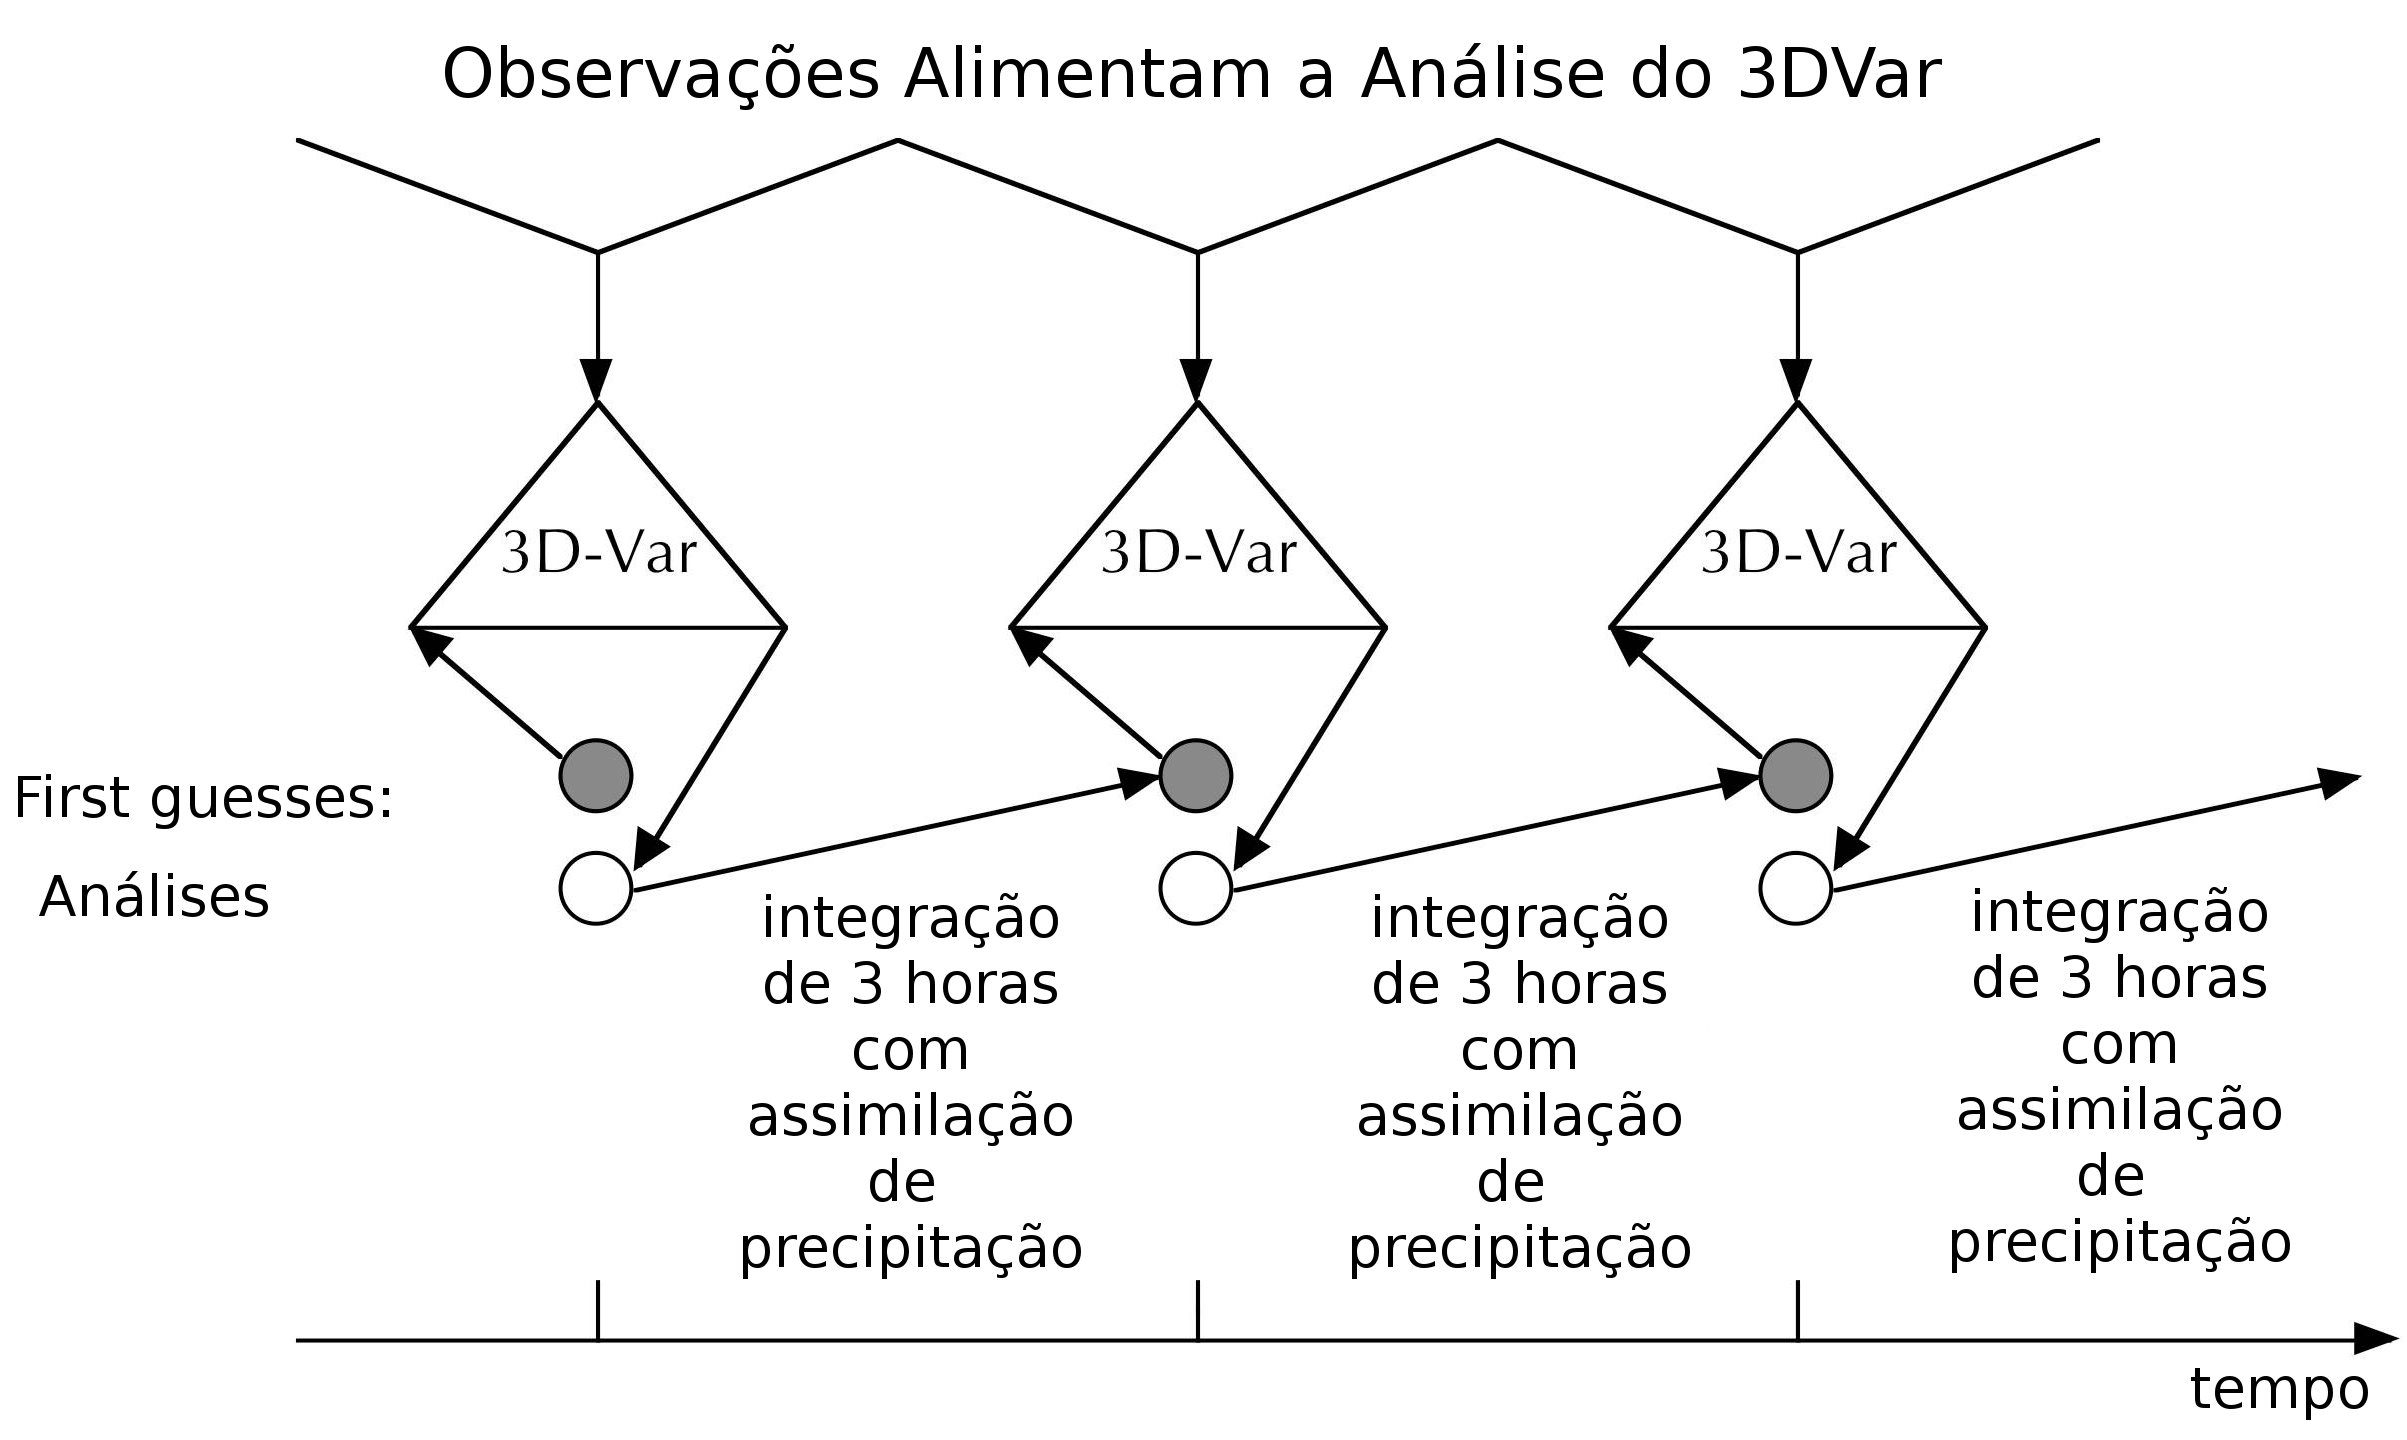
\includegraphics[height=7.5cm]{./figs/edas_pt.png}
\caption{Sistema de assimilação de dados EDAS/NCEP para um ciclo de 12Z.}
\FONTE{Adaptado de \citeonline{messingeretal06}}
\label{fig01}
\end{figure}

Sob este aspecto, geralmente nas primeiras horas de integração as variáveis dinâmicas estão se ajustando aos processos físicos/dinâmicos do modelo, isto é, as condições iniciais de superfície e atmosféricas estão entrando em balanço. Neste processo são filtradas as ondas espúrias (que são formadas a partir do desbalanço entre os campos de massa e vento do modelo) utilizando-se algum método de inicialização. Uma forma de se acelerar este processo de balanceamento, é incluir informações observadas e estimativas de superfície e/ou atmosfera, como precipitação, umidade e temperatura do solo. Isto faz com que seja reduzido o tempo de \textit{spin up} do modelo e permitindo que estas informações sejam propagadas pelo modelo ao longo do tempo de integração.

Tendo-se em vista que nas regiões tropicais do globo a convecção tem um papel dominante e sabendo-se que, em geral, os processos físicos associados à precipitação (convecção e microfísica) não são totalmente compreendidos, a modelagem atmosférica aplicada à estas regiões inclui uma série de aproximações. As parametrizações destes processos são inicialmente realizadas com estudos de campo que logo são modelados e então, extrapolados para o globo todo. Outros fatores como interações não lineares (principalmente sobre continente) com processos de superfície e camada limite, tornam difícil a previsão da precipitação. Consequentemente a convecção tende a não se formar nos horários e locais previstos por um modelo de mesoescala (como é o caso do modelo Eta). Por isso, estudos têm sido realizados com foco nas regiões tropicais com o objetivo de tentar minimizar os efeitos destas aproximações e/ou contorná-las. Uma forma de se atenuar este problema é incluir a precipitação no ciclo de assimilação de dados.

Diferentemente da IF, que se utiliza da inversão da parametrização convectiva para a assimilação da precipitação, a inclusão da precipitação no ciclo de assimilação de dados realizada neste trabalho é similar à técnica de \textit{nudging} em que as quantidades de umidade e temperatura são modificados à partir da comparação da precipitação produzida pelo modelo de previsão com a precipitação estimada/observada \cite{carrbaldwin91}. Além disso, uma das vantagens desta técnica está na sua implementação que não requer a modificação das equações prognósticas do modelo, pela inclusão de um termo extra para realizar o \textit{nudging} e também pode ser aplicada em conjunto com vários tipos de parametrização convectiva \cite{rogersetal05}.

\subsection{Área de Estudo}

A maior parte da AS está situada em uma área tropical extremamente chuvosa onde o potencial hídrico é um dos maiores do mundo. A precipitação exerce grande influência em diversos setores da atividade humana, como o planejamento agrícola, energético e hídrico, além de ser um fator determinante do clima e do tipo de vegetação característicos de diversas regiões. Além disso, o excesso e a escassez de precipitação podem proporcionar graves consequências à população, como episódios de enchentes e secas intensas, os quais acarretam perdas humanas e prejuízos materiais. Dessa forma, conhecer sua distribuição e quantidade sobre uma determinada área ou região, é crucial para melhorar o entendimento do ciclo hidrológico e de sua interação com as atividades do homem.

A AS – região de estudo deste trabalho, está situada entre os oceanos Pacífico e Atlântico e meridionalmente entre as latitudes de 10ºN e 60ºS. Esta é uma região sobre a qual atuam diversos tipos de sistemas atmosféricos reguladores do tempo e do clima e que têm importância devido à sua interação com a precipitação e a liberação de calor latente. Dentre eles, pode-se citar: a Zona de Convergência do Atlântico Sul (ZCAS), Zona de Convergência Intertropical (ZCIT), Jatos de Baixos e Altos Níveis, Alta da Bolívia e a Baixa do Chaco. Além disso, massas de ar e frentes atmosféricas entram e saem com frequência do continente. O deserto do Atacama, a cordilheira dos Andes, a floresta Amazônica e o Nordeste brasileiro, são exemplos também dos diferentes tipos de climas e regiões presentes na AS - \autoref{fig02} (adaptado de \citeonline{satyamurtyetal98}). Toda essa variedade de sistemas ambientais e meteorológicos em um continente situado numa zona tropical do globo, é consequência direta dos diferentes regimes de precipitação presentes na região. Além disso, há que se considerar também que, pelo fato de a AS estar situada no Hemisfério Sul (HS), as porções de terras e continentes nesta parte do globo são menores do que as porções de mares e oceanos. Esta situação é contrária ao que ocorre no Hemisfério Norte (HN). Nesta parte, a cobertura de radiossondagens e de equipamentos de monitoramento atmosférico sobre os continentes é muito maior e eficaz. Sobre o HS, este tipo de situação implica diretamente no uso de mais dados de satélites do que de observação em superfície.

\begin{figure}
\centering
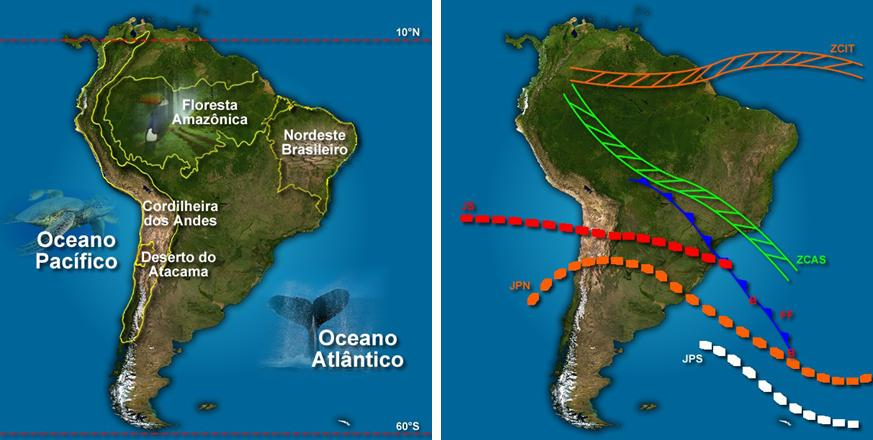
\includegraphics[height=7.5cm]{./figs/fig02.png}
\caption{As diferentes regiões e sistemas atmosféricos da América do Sul.}
\FONTE{Adaptado de \citeonline{satyamurtyetal98}}
\label{fig02}
\end{figure}

Grande parte dos regimes de chuva observados sobre os trópicos e em especial sobre a AS, é proveniente de um conjunto de sistemas meteorológicos denominados Sistemas Convectivos de Mesoescala (SCMs). Os SCMs são importantes fenômenos meteorológicos cuja principal característica é a sua organização em diversas formas, mas com escala espacial da ordem de centenas a milhares de quilômetros de extensão. Os Complexos Convectivos de Mesoescala (CCMs) são uma classificação dos SCMs e representam sistemas convectivos que produzem alterações significativas na dinâmica de mesoescala, sendo na geração e distribuição de calor latente, nas alterações de estabilidade vertical e redistribuição de umidade e, principalmente, na quantidade de radiação que entra e sai da atmosfera, devido à cobertura de nuvens associados a esses sistemas (\cite{velascofritsch87}).

Diversos autores como \citeonline{menezessilvadias04}, \citeonline{herdiesetal07} e mais recentemente \citeonline{rozantecavalcanti07}, realizaram estudos numéricos sobre a simulação de CCM sobre a América do Sul, especialmente à leste dos Andes sobre o norte da Argentina. Nestes estudos, além da quantificação e determinação da climatologia dos CCMs sobre a AS, avaliou-se o impacto da assimilação de dados do projeto de campo do SALLJEX na simulação de sistemas convectivos de mesoescala. Também  se procurou as configurações mais adequadas para a simulação dos CCMs sobre o norte da Argentina. Estes tipos de estudos tem sua importância devido ao fato de que os CCMs são importantes fenômenos meteorológicos causadores de tempo e clima severos e que contribuem significativamente para a variação dos níveis pluviométricos, principalmente sobre as regiões tropicais e que podem estar associados a chuvas muito fortes, intensas rajadas de ventos, descargas elétricas atmosféricas, granizo e até tornados \cite{maddox80}; \cite{menezessilvadias04}.

Historicamente, a primeira definição formal de CCM foi introduzida por \citeonline{maddox80} para o Hemisfério Norte (HN). Mais tarde outros autores utilizaram esta definição para estudar outros casos de CCMs em partes diferentes do globo, como \citeonline{velascofritsch87}, na América do Sul. Segundo os critérios de \citeauthoronline{maddox80}, os CCMs podem ser classificados de acordo com suas características físicas: forma, tamanho e ciclo de vida. Quanto à forma, o CCM deve ser de formato circular, com excentricidade maior do que 0,7 (considerando-se a razão entre o eixo menor e o eixo maior - \autoref{fig03}). Quanto ao tamanho, o CCM deve apresentar uma cobertura de nuvens com temperaturas no infravermelho menores do que -32ºC e com área de 100.000 km². Na região mais interna da nuvem, as temperaturas devem ser mais frias (menores do que -52ºC) e com área em torno de 50.000 km². Quanto ao ciclo de vida, o CCM deve apresentar as características de tamanho persistentes a um período superior a 6 horas.

\begin{figure}[!hpb]
\centering
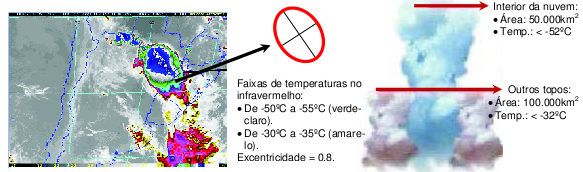
\includegraphics[height=4.5cm]{./figs/fig08.png}
\caption{À esquerda: imagem no infravermelho do satélite GOES (20030123, às 02:09 UTC). Ao centro: característica da excentricidade do CCM ocorrido nesta data. À direita: secção transversal de uma nuvem do gênero \textit{Cumulonimbus} durante um CCM.}
\FONTE{\citeonline{rozante08}}
\label{fig03}
\end{figure}

Todas estas características são semelhantes em escalas espaciais meso-a (ou meso-$\alpha$, de 250 a 2500 km de extensão e escala de tempo de 6 horas) e meso-b (ou meso-$\beta$, de 25 a 250 km de extensão e escala de tempo inferior a 6 horas).

Tipicamente, os CCMs são caracterizados por um conjunto de nuvens do gênero \textit{Cumulonimbus} cobertas por uma camada densa de nuvens do gênero \textit{Cirrus} e são facilmente identificados em imagens de satélites \cite{silvadias87}. O ciclo de vida dos CCMs é habitualmente noturno, ou seja, sua máxima extensão ocorre durante a madrugada \cite{velascofritsch87}, sendo o fim desse ciclo na metade do dia subsequente. Estas características dos CCMs tropicais e subtropicais são semelhantes em ambos os hemisférios (HN e HS) e estão sumarizadas na \autoref{tab01}.

\begin{table}
\caption{Resumo das Características dos CCMs.}
\label{tab01}
\centering
\begin{tabular}{c|p{12cm}l}
\hline
\multicolumn{2}{c}{Caractarísticas}                                                 \\
\hline
Forma                                       & Circular: excentricidade maior do que 0,7.\\
\hline
\multirow{4}{2cm}{Tamanho}                  & Nuvens: topo com temperaturas \\
                                            & inferiores a -32ºC e cobertura \\
                                            & com área de $\sim$ 100.000 km²; \\
                                            & Parte interna: temperaturas inferiores a -52ºC e área de 50.000 km².         \\
\hline
\multirow{3}{2cm}{Ciclo de Vida}            & As características do tamanho devem persistir por mais do que 6 horas;   \\
                                            & Habitualmente noturno, com máxima extensão na madrugada.                \\
\hline
\multirow{3}{2cm}{Escala}                   & Meso-$\alpha$: 250 a 2500 km de extensão e duração igual ou superior a 6 horas;      \\
                                            & Meso-$\beta$: 25 a 250 km de extensão e duração inferior a 6 horas. \\
\hline
\multirow{4}{2cm}{Locais de Ocorrência} & Estados Unidos (HN);                  \\
                                            & Pacífico Oeste (HN);              \\
                                            & África (HS);                      \\
                                            & América do Sul (HS);              \\
\hline
\end{tabular}
\FONTE{Adaptado de \citeonline{velascofritsch87}}
\end{table}

No Brasil os CCMs ocorrem mais frequentemente sobre a região Sul, havendo também referências de se deslocarem para as regiões Sudeste e Centro-Oeste, podendo ocorrer em todas as estações do ano \cite{silvadias96}.

Na AS, o principal mecanismo de transporte de umidade da região amazônica para a região sul da AS, é o JBN. O JBN é frequentemente associado ao transporte de umidade e consequente formação da convecção de grande parte dos SCMs \cite{ferreiraetal03} que ocorrem sobre a região centro-sul da AS. O transporte de umidade da região amazônica em direção à região sul da AS, geralmente condensa e precipita na região de saída do JBN, produzindo fortes correntes descendentes sob o núcleo dos SCMs, com o máximo de precipitação durante a noite \cite{noguesetal00}. Esta característica é predominante em meses de verão, sendo que em meses de inverno, boa parte da umidade que condensa e precipita sobre o sul do continente é transportada pelos ventos alísios no norte do nordeste do continente. Na \autoref{fig04} é mostrado um modelo conceitual dos JBN e sua associação com a formação dos CCMs \cite{marengoetal04}.

\begin{figure}
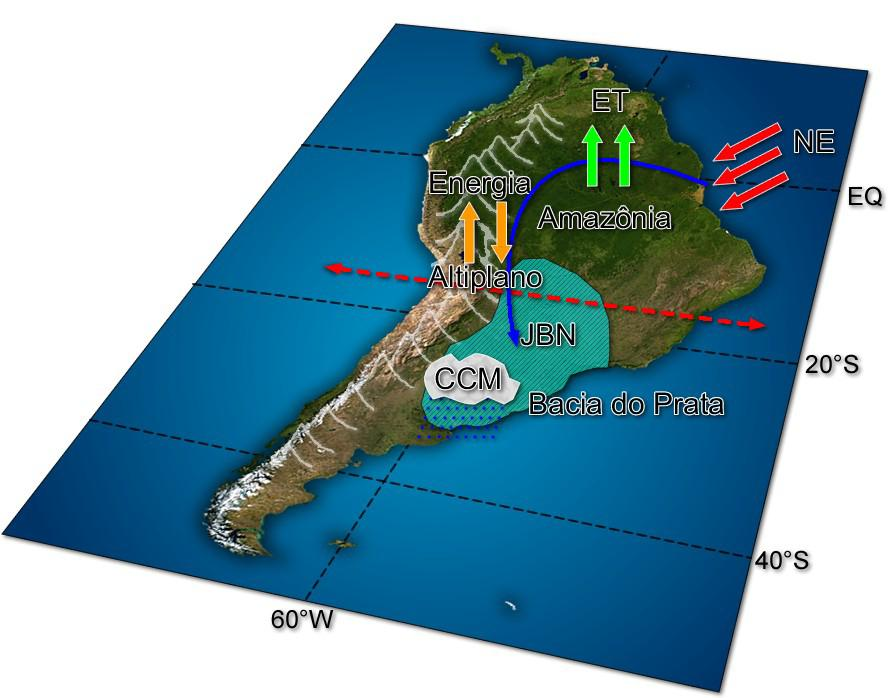
\includegraphics[height=10cm]{./figs/fig10.png}
\caption{Modelo Conceitual dos JBN. Na figura: ET - evapotranspiração do vapor d'água da floresta mazônica; JBN - Jato de Baixos Níveis que transportam a umidade e CCM - Complexo Convectivo de Mesoescala; NE - Ventos Alísios no norte do nordeste do continente.}
\FONTE{adaptado de \citeonline{marengoetal04}}
\label{fig04}
\end{figure}

Portanto, para prever e simular as alterações dinâmicas e atmosféricas causadas por esses sistemas convectivos tais como as mudanças de fase da água, os efeitos dos processos radiativos (de onda curta e longa), as trocas turbulentas de calor, momentum e vapor d'água entre a superfície e a atmosfera e os transportes turbulentos de calor, umidade e momentum na atmosfera, exigem não apenas modelos modernos e computadores de alto desempenho, mas principalmente o aprimoramento do uso das observações disponíveis para que a condição inicial dos modelo de PNT seja a mais realística possível e, com essa análise mais acurada, fazer estudos diagnósticos que permitam o entendimento da dinâmica dos mesmos.

\section{Objetivos}
\label{ss:objetivos} 

O objetivo principal deste trabalho é avaliar o impacto da inclusão de dados de precipitação no sistema de assimilação de dados regional do CPTEC.

Além disso, como objetivos específicos, buscou-se avaliar também:

\begin{enumerate}
\item O impacto da assimilação de dados de precipitação no desempenho do modelo Eta durante o mês de Janeiro de 2003;
\item O impacto da assimilação de dados de precipitação em um estudo de caso de CCM ocorrido em janeiro de 2003: identificação e simulação (ciclo de vida, posicionamento e intensidade);
\end{enumerate}

Para este propósito foi utilizado o sistema de assimilação de dados RPSAS junto com o modelo regional de mesoescala Eta. Dados de precipitação provenientes do \textit{Tropical Rainfall Measuring Mission} (TRMM) foram usados neste estudo. Esta avaliação teve também o intuito de verificar como a assimilação de precipitação no sistema Eta+RPSAS melhora a qualidade das análises e previsões regionais. O estudo foi desenvolvido para o mês de janeiro de 2003, período em que se têm dados observados do SALLJEX, com especial atenção ao período em que houve ocorrência dos CCM (18 a 23 de janeiro de 2003).

No \autoref{ss:cap2} deste trabalho são apresentados os componentes do sistema de assimilação de dados RPSAS que foram utilizados nos experimentos, considerando-se também as principais características do modelo Eta, método de assimilação e o conjunto de dados utilizado. No \autoref{ss:cap3} apresentam-se os resultados do período de análise, avaliação do desempenho do sistema Eta+RPSAS e o impacto da assimilação de  precipitação nas previsões do modelo Eta. No \autoref{ss:cap4} apresenta-se um estudo de caso de CCM. Finalmente, no \autoref{ss:cap5}, são apresentadas as conclusões e sugestões de trabalhos futuros.
